\documentclass[main.tex]{subfiles} % Subfile-Class


% ============================================================================== %
%                            Subfile document                                    %
% ============================================================================== %

\begin{document}

\section{Konzepterstellung Antriebe}~\label{appendix:Antriebe}

Dieser Abschnitt befasst sich mit den Antrieben des Pfadfinders. Dabei werden
sowohl verschiedene Motorenkonzepte diskutiert, als auch potenziell
Einsatzfähige Motoren herausgesucht. Im Abschluss wird noch Konzeptionell
zusammengefasst, wie diese Antriebe anzusteuern sind.

% ===================================================
\subsection*{Anforderungen}

\begin{description}
    \item[Beschleunigung] Eine selbstgesetzte, ehrgeizige Anforderung an das Roboter ist,
          den Roboter innerhalb einer Sekunde auf eine Geschwindigkeit von $2 \frac{m}{s}
          $ beschleunigen zu können.

    \item[Gewicht] Gewicht ist, wie bei allen anderen Baugruppen ebenfalls, ein sehr
          kritischer Punkt bei der Entwicklung des Pfadfinders. Als
          \textit{Gewichtsbudget} wurde für die Antriebseinheit festgelegt, dass das
          Gewicht nicht grösser als total $500 g$ sein sollte.

    \item[Kosten] Das Budget dieses Projekts ist sehr beschränkt. Antriebe können hierbei
          einen wesentlichen Kostenpunkt darstellen, weshalb dem Antrieb inklusive der
          Ansteuerung und Räder ein Budget von $100 CHF$ zugewiesen wurde.

    \item[Nennspannung] Die benötigte Nennspannung des Boardnetzes richtet sich
          mehrheitlich nach der benötigten Spannung der Motoren. Wie im
          Kapitel~\ref{appendix:Bordnetz} bereits erwähnt wurde, würde eine Spannung von
          24V ein nicht umsetzbares Gewicht darstellen. Daher beträgt die Maximalspannung
          für Motoren hier 12V Nennspannung.

    \item[Technologie] Die Ansteuerung der Motoren ist mit geeigneten Treibern in den
          meisten Fällen relativ einfach umzusetzen. Aufgrund bestehender Erfahrungswerte
          sollen vorzüglich Schrittmotoren eingesetzt werden.

    \item[Schnittstelle] Die Schnittstelle zur Ansteuerung der Motoren soll einem einfach
          umzusetzenden Standard entsprechen. Das betrifft die Ansteuerung über bekannte
          Bus-Protokolle wie $I^2C$, $SPI$, $UART$ oder aber auch PWM- oder Step/Dir
          Interfaces.

\end{description}

Die Anforderungen an den Akku schliessen aufgrund der 12V-Boardnetzspannung
Industrietaugliche 24V-Motoren bereits aus. Diese sind zwar sehr robust,
allerdings in den meisten Fällen auch sehr schwer.

\subsubsection*{Leistungsanforderungen an Motoren}

==============================================================================
Text Yanik zu Dimensionierung
==============================================================================

% ===================================================
\subsection*{Konzeption}

Aus den Leistungsanforderungen an die Motoren heraus lässt sich auf dem Markt
schauen, welche Motoren potenziell zur Verfügung stehen. Diese lassen sich
wiederum in den Kriterien Kosten, Gewicht, Leistung und Entwicklungsaufwand
gegeneinander vergleichen.

\subsubsection*{Konzept 1 - Bipolarer Schrittmotor} % =========

Die Wahl für einen bipolaren Schrittmotor fällt, da er bei gleichem Gewicht
eine grössere Ausnutzung der Spulen bringt - woraus eine höhere Leistung bei
gleichem Gewicht im Vergleich zu einem unipolaren Schrittmotoren resultiert.

Ein Vergleich verschiedener Schrittmotoren hat gezeigt, dass Schrittmotoren,
welche sich in einem Nennstrombereich von $1.2A$ bis $2A$ in einem Bereich
befinden, welche den Leistungsanforderungen bereits ohne Zwischengetriebe
genügen können.

Typische, günstige Vertreter aus dieser Reihe sind die in
Tabelle~\ref{tab:Schrittmotoren_different} aufgeführten.

\begin{table}[h]
    \centering
    \begin{tabular}{|p{2cm}|p{3cm}|p{2cm}|p{1cm}|p{1cm}|p{1cm}|p{1.5cm}|}
        \hline
        Hersteller           & Herst. Nr      & Distributor & $I_{nenn} $ [A] & $U_{nenn}$ [V] & Preis [CHF] & Gewicht [kg] \\ \hline
        Olimex LTD           & SM-42HB34F08AB & DigiKey.ch  & 1.33            & 12             & 9.36        & 0.400        \\ \hline
        DFRobot              & FIT0278        & DigiKey.ch  & 1.7             & 3.4            & 12          & 0.269        \\ \hline
        SparkFun Electronics & ROB-10846      & DigiKey.ch  & 1.7             & 3              & 16.77       & 0.356        \\ \hline
    \end{tabular}
    \caption{Verschiedene Schrittmotoren}
    \label{tab:Schrittmotoren_different}
\end{table}

Dieser Vergleich zeigt, dass sich eigentlich nur der Motor \textit{FIT0278} von
\textit{DFRobot} in einem akzeptablen Gewichts-Leisungs-Verhältnis befindet.
Preisgünstig sind alle aufgeführten Motoren.

Die Motoren sollen über eingekaufte Treiber angesteuert werden. Zwar ist eine
Eigenentwicklung eines Motorentreibers mit nicht allzu viel Aufwand umzusetzen,
jedoch sind fertige Treiber-Endstufen sehr günstig zu haben und einfach
anzusteuern. Ein Team-Mitglied kann auf Erfahrung aus seinem beruflichen Umfeld
zurückgreifen bei der Ansteuerung des Schrittmotorentreibers \textit{TMC5240}
von \textit{ADI-Trinamic}. Diese Treiber stehen darüber hinaus für dieses
Projekt in zweifacher Ausführung zur Verfügung. Der Vergleich dieses Treibers
mit einem einfach anzusteuernden Treibers zeigt die
Tabelle~\ref{tab:Schrittmotorentreiber_different}.

\begin{table}[h]
    \centering
    \begin{tabular}{|p{2cm}|p{3cm}|p{2cm}|p{1cm}|p{1cm}|p{1cm}|p{1.5cm}|}
        \hline
        Hersteller & Herst. Nr    & Distributor & $I_{nenn} $ [A] & $U_{nenn}$ [V] & Preis [CHF] & Gewicht [kg] \\ \hline
        ADI        & TMC5240-EVAL & Komax AG    & 2               & 36             & 63          & 0.036        \\ \hline
        ACT Motor  & ACT DM430    & reichelt.ch & 3               & 32             & 17.42       & 0.180        \\ \hline
    \end{tabular}
    \caption{Verschiedene Schrittmotorentreiber}
    \label{tab:Schrittmotorentreiber_different}
\end{table}

\subsubsection*{Konzept 2 - Radnabenmotor} % =========

Es gibt fertig zu kaufende Radnaben auf dem Markt, welche zum Teil bereits
sowohl Endstufen als auch eine Ansteuerung beinhalten.

Als Beispiel zu nennen wäre da der folgende:

\begin{table}[h]
    \centering
    \begin{tabular}{|p{2cm}|p{3cm}|p{2cm}|p{1cm}|p{1cm}|p{1cm}|p{1.5cm}|}
        \hline
        Hersteller & Herst. Nr & Distributor & $I_{nenn} $ [A] & $U_{nenn}$ [V] & Preis [CHF] & Gewicht [kg] \\ \hline
        DFRobot    & FIT1001   & DigiKey.ch  & 0.5             & 14.4           & 25.71       & 0. 216       \\ \hline
    \end{tabular}
    \caption{Radnabenmotor DFRobot}
\end{table}

Der gezeigte Motor ist einfach über den UART-Bus anzusteuern, günstig, leicht
und besitzt einen integrierten Encoder. Ein grosser Nachteil dagegen ist, dass
mit diesem Motor das ehrgeizige Ziel einer Beschleunigung von $2 \frac{m}{s^2}$
voraussichtlich nicht erreicht werden kann.

\subsubsection*{Konzept 3 - BLDC-Motor} % =========

BLDC Motoren bieten den grossen Vorteil, dass sie bei kleinem Gewicht eine hohe
Leistung erreichen können. Ihr Drehmoment hingegen ist eher gering - woraus die
Notwendigkeit an ein Zwischengetriebe besteht. Dieses Zwischengetriebe treibt
das Gewicht des Antriebs weiter in die Höhe. BLDC Motoren kommen darüber hinaus
häufig mit einem höheren Preis daher.

Die nachfolgende Tabelle zeigt eine Aufstellung verschiedener Motoren, welche
in Frage kommen könnten.

% YANIK FRAGEN DER DFROBOT KÖNNTE NOCH SPANNEND SEIN !!!!!!!!!!!!!!!!!!!!!!!!!!!!!!!!!!!!!!!!

\begin{table}[h]
    \centering
    \begin{tabular}{|p{2cm}|p{3cm}|p{2cm}|p{1cm}|p{1cm}|p{1cm}|p{1.5cm}|}
        \hline
        Hersteller      & Herst. Nr     & Distributor & $I_{nenn} $ [A] & $U_{nenn}$ [V] & Preis [CHF] & Gewicht [kg] \\ \hline
        DFRobot         & FIT0441       & DigiKey.ch  & 0.7             & 12             & 17.11       & 0.070        \\ \hline
        Lin Engineering & BL17E19-01-RO & DigiKey.ch  &                 & 24             & 79.18       & 0.320        \\ \hline
    \end{tabular}
    \caption{Radnabenmotor DFRobot}
\end{table}

Der Motor von DFRobot wird zwar mit seiner Geschwindigkeit von maximal $159
    \frac{1}{min}$ die gewünschte Drehzahl zwar nicht erreichen, das geringe
Gewicht bei entsprechender Leistung sowie sein bereits integrierten Treiber
macht diesen Antrieb allerdings trotzdem Wert, im Detail beurteilt zu werden.

Generell lässt sich sagen, die Suche nach Bauteilen hat ergeben, dass
BLDC-Motoren eine höhere Nennspannung benötigen, als mit dem Dimensionierten
Akku-Pack zur Verfügung gestellt werden kann. Natürlich arbeiten Motorentreiber
als Stromquellen, allerdings sind Motoren im entsprechend benötigten
Leistungsbereich schnell zu teuer und schwer.

Generell lassen sich BLDC-Motoren, ähnlich wie die Schrittmotoren, über einen
selbst entwickelten Treiber ansteuern, allerdings sind fertige Motorensteuerung
ebenfalls unschlagbar günstig und über ein PWM-Interface sehr einfach
anzusteuern. Als Vertreter dieser Produktgruppe ist der folgende zu nennen.

\begin{table}[h]
    \centering
    \begin{tabular}{|p{2cm}|p{3cm}|p{2cm}|p{1cm}|p{1cm}|p{1cm}|p{1.5cm}|}
        \hline
        Hersteller & Herst. Nr    & Distributor & $I_{nenn} $ [A] & $U_{nenn}$ [V] & Preis [CHF] & Gewicht [kg] \\ \hline
        ACT Motor  & BLDC-8015A-5 & reichelt.ch & 15              & 50             & 39.1        & 0.432        \\ \hline
    \end{tabular}
    \caption{BLDC-Treiber}
\end{table}

\subsubsection*{Fazit und Entscheid aus der Konzeptionsphase}  % =========

In der Gruppe ist der Entscheid darauf gefallen, den Schrittmotor von DFRobot,
gezeigt in Abbildung~\ref{fig:DFROBOT_FIT0278}, in Kombination mit den
\textit{Trinamic}-Schrittmotorentreibern, gezeigt in
Abbildung~\ref{fig:TMC5240_EVAL}, genauer zu analysieren und zu verfolgen. Als
\textit{Plan-B}, auch für den Fall, dass das gewünschte Gewicht nicht
eingehalten werden kann, soll der Radnabenmotor, ebenfalls von DFRobot,
evaluiert werden. Damit können zwar nicht zwingend die gewünschten
Geschwindigkeits- und Beschleunigungswerte erreicht werden, dafür ist seine
Ansteuerung sehr einfach, sie haben ihre Treiber bereits integriert und dazu
sind sie auch leicht.

\begin{figure}[h!]
    \centering
    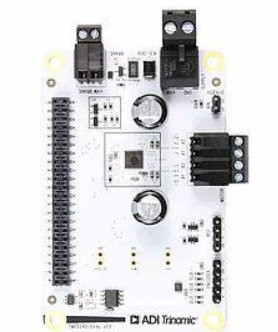
\includegraphics[width=0.25\textwidth]{./fig_Antriebe/TMC_5240_EVAL.png}
    \caption{TMC 5240 Evaluation-Board}~\label{fig:TMC5240_EVAL}
\end{figure}

\begin{figure}[h!]
    \centering
    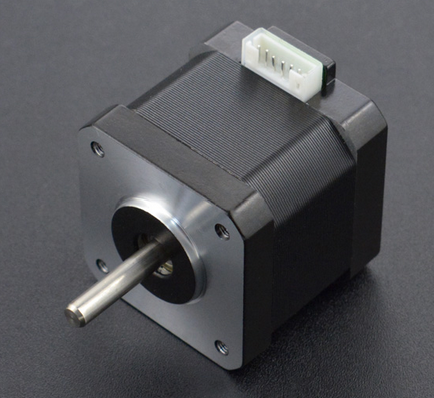
\includegraphics[width=0.25\textwidth]{./fig_Antriebe/DFRobot_Stepper_FIT0278.png}
    \caption{DFROBOT FIT0278 Schrittmotor}~\label{fig:DFROBOT_FIT0278}
\end{figure}

Geregelt werden soll dieser Motor von einem echtzeitfähigen Mikroprozessor,
welcher ebenfalls über die Sensordaten des Liniensensors verfügt. Der Antrieb
soll auf das Feedback eben dieses Sensors geregelt werden. Dies ist auf
Abbildung~\ref{fig:RTC_Trinamic_Konzept} nochmals verdeutlicht.

\begin{figure}[h!]
    \centering
    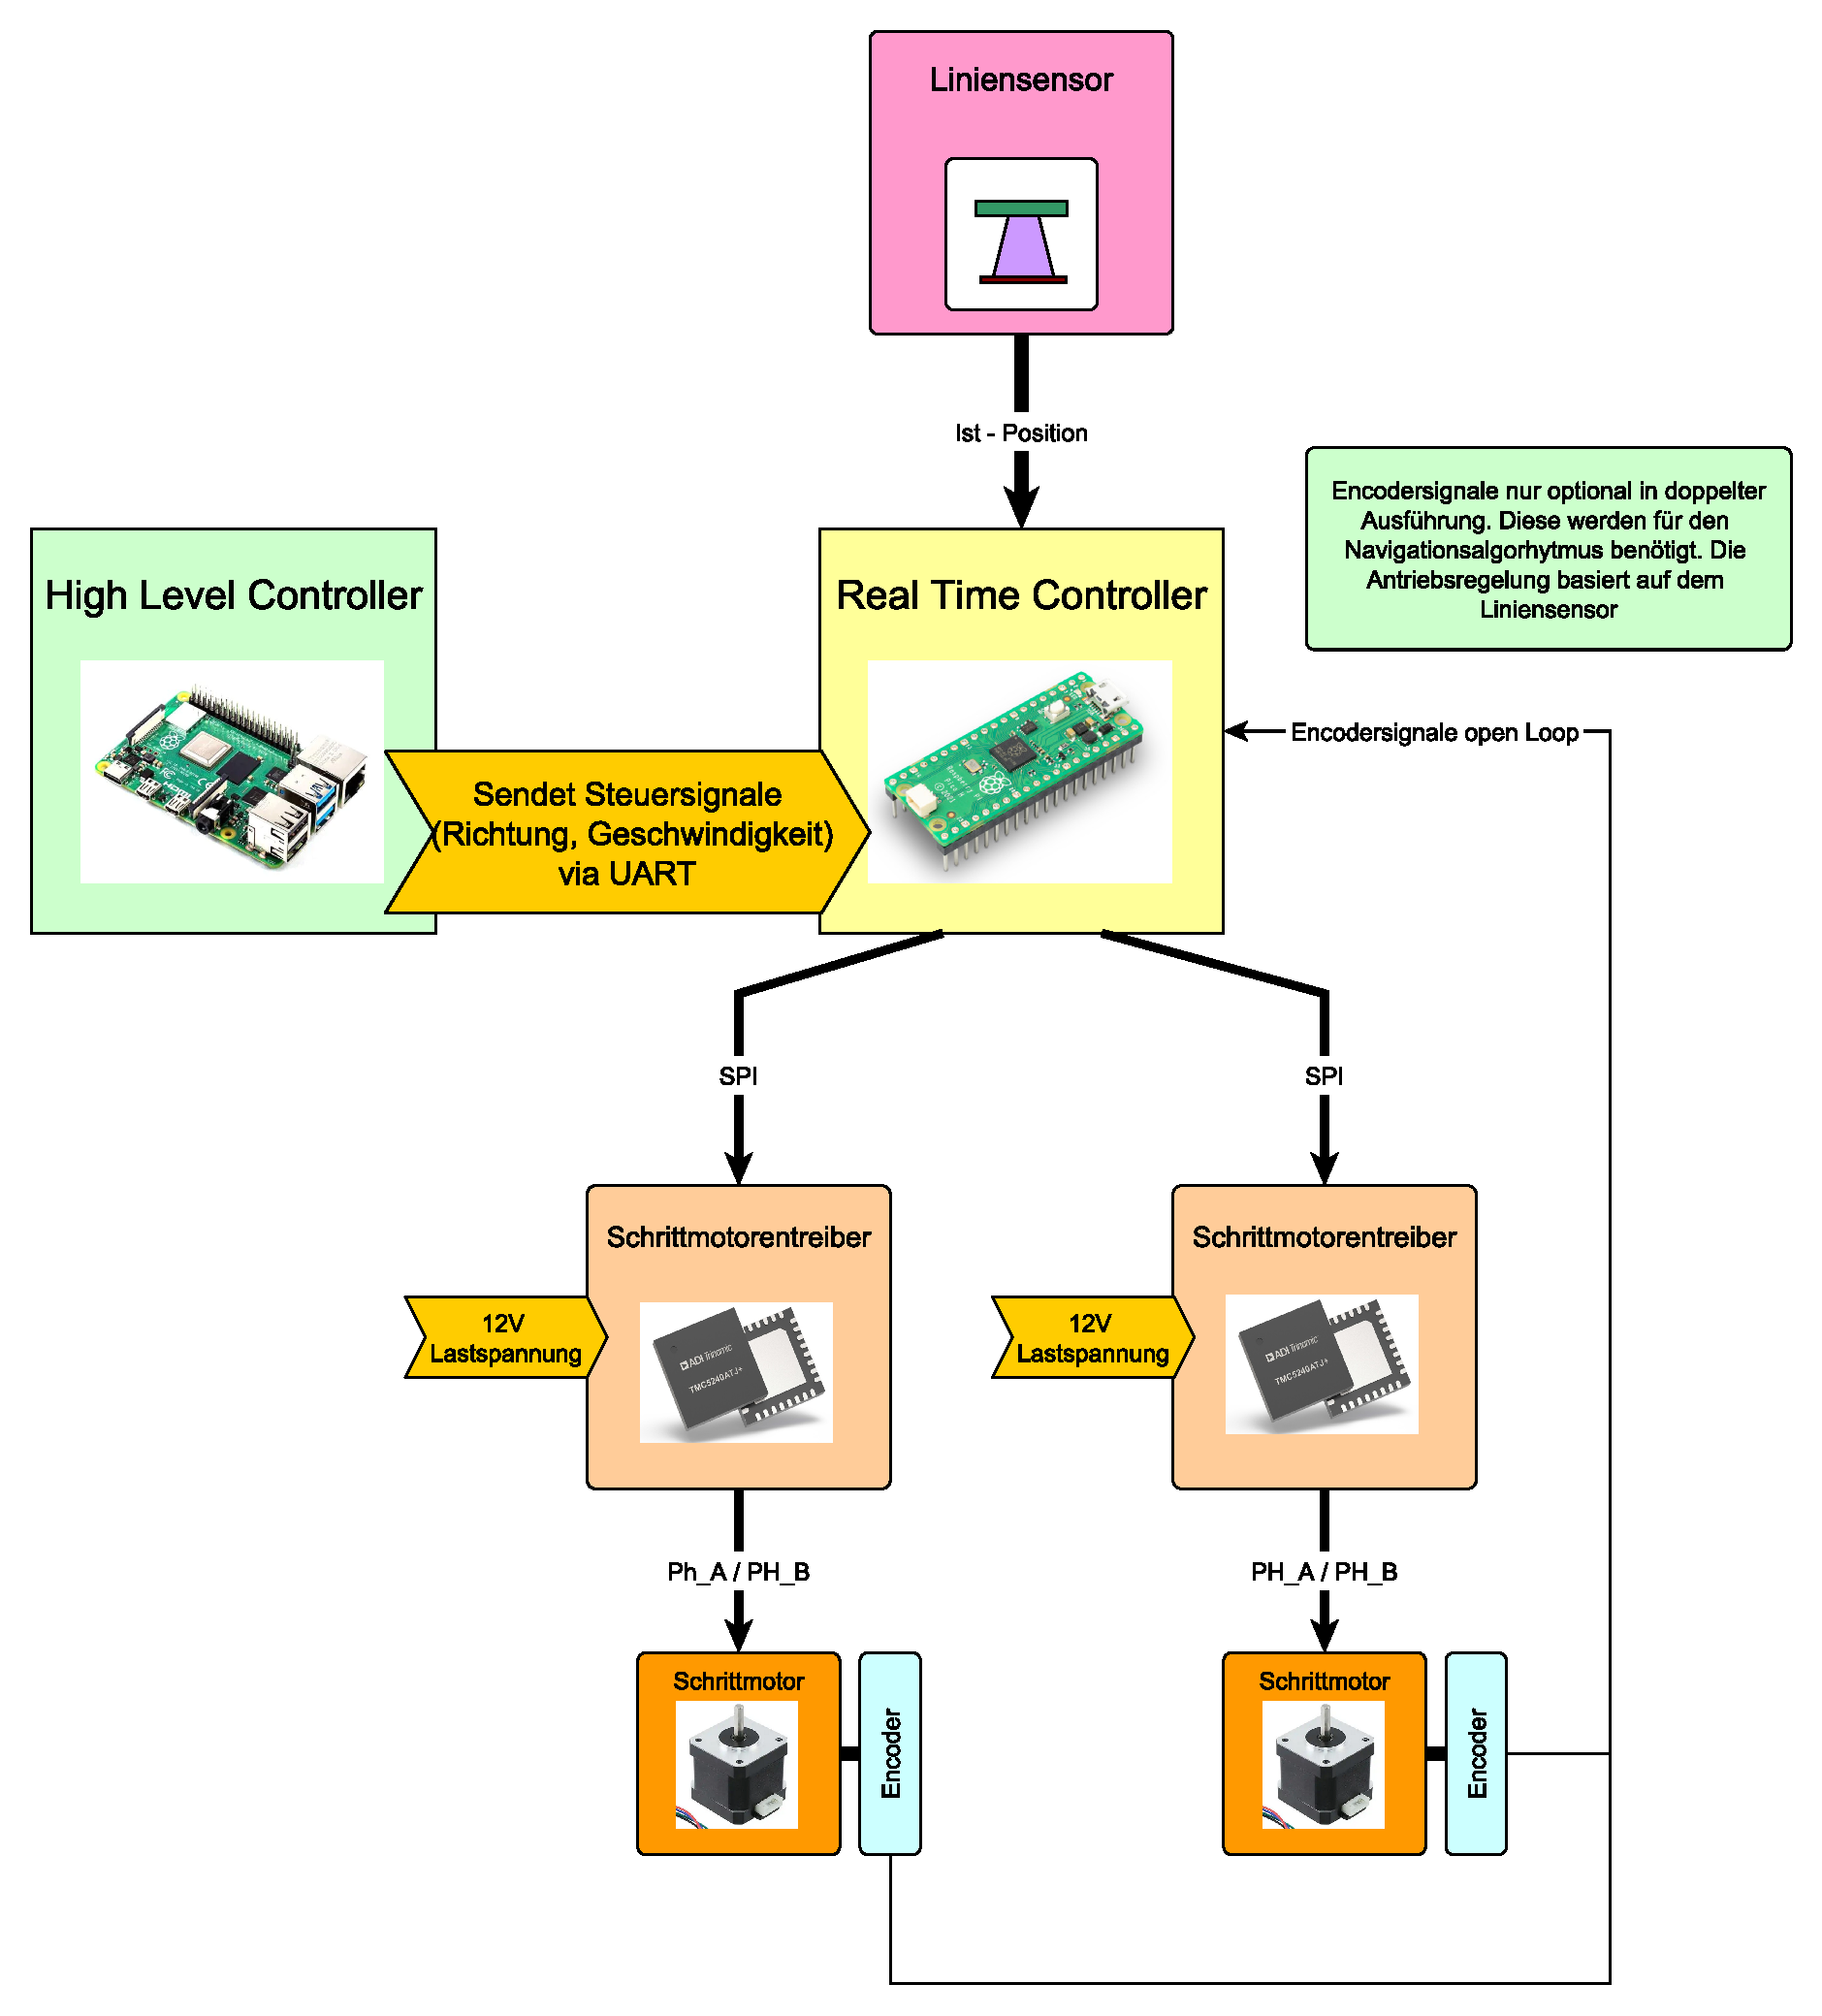
\includegraphics[width=0.75\textwidth]{./fig_Antriebe/Konzept_RTC_Trinamic.pdf}
    \caption{Konzept für die Ansteuerung der Schrittmotoren}~\label{fig:RTC_Trinamic_Konzept}
\end{figure}

Zusätzlich wird noch mindestens ein Encoder vorgesehen, welcher mit einer
einfachen Lochscheibe und einer Gabellichtschranke umgesetzt wird. Dieser hat
allerdings keine Anwendung auf die Fahrzeugregelung. Mit ihm soll lediglich die
zurückgelegte Strecke erfasst werden.

Die gewählten Treiber liessen sich direkt über den High-Level-Controller
ansteuern. Die Antriebsregelung wurde aber bewusst auf einen Mikroprozessor
verschoben, um dem Ansatz der Gewaltentrennung gerecht zu werden. So gibt es
einen Echtzeitfähigen Prozessor, welcher sich ausschliesslich mit der
Positionsregelung befasst, während der High-Level-Controller lediglich
Entscheidungen trifft, in welche Richtung gefahren werden muss.

\end{document}
